\documentclass[9pt,twocolumn,twoside]{../../styles/osajnl}
\usepackage{fancyvrb}
\journal{i524} 

\title{Optical Character Recognition}

\author[1]{Saber Sheybani}
\author[1]{Sushmita Sivaprasad}


\affil[1]{School of Informatics and Computing, Bloomington, IN 47408, U.S.A.}


\affil[*]{Corresponding authors: sheybani@umail.iu.edu,sushsiva@umail.iu.edu}

\dates{project-000, \today}

\ociscodes{OCR,ansible,classification}

% replace this with your url in github/gitlab
\doi{\url{https://github.com/SushmitaSivaprasad/sp17-i524/tree/master/project/S17-IR-P012/report/report.pdf}}


\begin{abstract}
Optical Character Recognition is a technology for converting images
into machine encoded text format. In this project, the input data is
in PNG format and our goal is to recognize the words/letters in the
image as accurately as possible and convert the dataset into TXT
format. The heart of OCR is a classification algorithm which will be
implemented using Python programming language. The algorithm will be
deployed using the Ansible technology \cite{www-ansible}  to remote virtual clusters.
\newline
\end{abstract}



\begin{document}

\maketitle

\section{1.Introduction}

This project proposal provides an overview on how we plan on
implmenting the OCR technology. It gives a background on the kind of
technology that has been used , delving into some of the basic
concepts used in the implentation process.We have also discussed some
important applications of this technology in the real world.

\section{2.Background}
\subsection{2.1 OCR Technology}  
Optical Character Recognition is a technology which is used to convert
different types of documents that can be in the form of scanned papers
(raster images) or PDF into an editable and searchable form  \cite{www-ocr}. The
images can be in either the basic black \& white or multicolored.  The
technology first analyzes the structure of the document and divides it
into smaller segments. Finally, individual characters are singled out
one by one and fed to a classification algorithm which will return the
closest letter that the individual character could possibly be
identified with.

\subsection{2.2 Ansible} 
Ansible is an IT automation tool. It uses YAML in order to issue the
state of the server \cite{www-ocr}. Ansible implements the internal command that
is required to reach that state which depends on the operating
system. The ansible playbook which consists of these internal commands
can be applied across any server or service. There is no requirement
to instal an additional software on the target system as the commands
are run over an SSH session.

\subsection{2.3 Feed Forward Neural Networks}
Artificial Neural Network is a paradigm in computing, inspired by the
structure of biological nervous systems. It consists of a network of
processing units, where the output of each unit is a nonlinear
function of its weighted inputs that come from other units. Such
network can be trained to solve different kinds of problems, including
classification and clustering. A feed forward neural networks is one
in which the neurons are organized in a number of layers and each
layer only feeds to the next one, but not to the previous one (no
feedback). However, in a back-propagation process, the errors from one
iteration of classification will be fed back from the output to the
network, in order to modify and improve the network for next
iterations.

\section{3.Ansible Deployment}
We will be using Ansible \cite{www-ansible} for running the OCR algorithm. The jobs
will be collected and organized in a Playbook \cite{www-ansible-playbook} and run on virtual
clusters provided by Chameleon Cloud \cite{www-chameleoncloud}.  The tasks will include
Installing the essential libraries on the remote machine and running
the program.

\section{4.OCR Implementation}

Optical Character Recognition have already been developed in numerous
ways, focusing on different goals. For our purpose, various
classification algorithms such as K-Nearest Neighbor and Neural
Network (multilayer perceptron) can be used. For this project, a
feedforward, back-propagation Neural Network will be used. The steps
are as follows: Preprocessing: The input images need to be segmented
into units that each of them keep only one glyph (symbol). Also, the
colored or grayscale images will be binarized.  Feature extraction:
The glyphs will be decomposed into features like lines, closed loops,
line direction, and line intersections.  Character recognition: The
image features will be fed to the neural network and they will be
compared with stored glyph features and the nearest match will be
chosen, after multiple iterations of classification by the network.

\section{5.Pre processing the data}


\textbf{Preprocessing Techniques} :

Preprocessing is required on the raw images that we are using to
filter out the required subject and distinguish from any other
unwanted objects from the image such as watermarks, background
subjects etc. We have conducted different preprocessing techniques in
order to remove noise and convert the image into a grey scale format
as color images requires more complex methods of processing

\subsection{5.1 Binarization}

Otsu’s method \cite{otsu1975threshold} Otsu’s method concludes finding
the best intensity threshold to separate two classes, often background
vs foreground but not always. The algorithm tries to find a separation
point that has the minimum weighted within class variance.  If the
input images are grayscale, the algorithm will simply find a threshold
that any intensity below that will be considered as the background and
the intensity of the corresponding pixels will be rounded to
zero. Similarly, the intensities above the threshold will be rounded
to 1. The resulting image (array) will be binary.  .
 
\subsection{5.2 Noise Reduction Techniques}

Noise reduction is done for extracting out any unwanted bit-pattern,
there are linear as well as non-linear techniques for this.  Linear :
In this method is used to remove any isolated pixel noise from the
image. Here the required output filter is taken as a linear
combination of the neighborhood pixels Non- Linear : These kind of
filters are used to replace the value of a particular pixel in order
to remove any kind of impulse noise

\subsection{5.3 Histogram Based Method}

It gives a value to the intensity of the pixel and plot it on a
histogram , where darker the image , more the data points would be on
the left and center of the histogram . Lighter the image , more the
data points would be on the right side of the histogram. Using a
histogram equalization method the contrast on the image can be
improved in this case. In the histogram equalization method , an image
is divided into blocks of pixels and an histogram equalization is
done.  This allows us to distinguish the images we actually require
from the other background images . It allows us to enhance the
visibility of the characters’ present on the image.

\subsection{5.4 Median Filter}
It is a non-linear noise reduction technique , it is a low pass
filter. In this case the pixel values are taken for an area on the
image and an average of the pixel value is taken and assigned to the
center pixel in that area. It is an effective means for removing the
salt and pepper noise which are random lines occurring on the image
due to poor quality of the picture or if the image wasn’t scanned
well.\cite{medianfilterpreprocessing}Figure 2 shows the result of
applying a median filter on a scanned image, we can see the reduction
in dots and other marks on the image, making it more smooth and
usable.
 

\begin{figure}
\centering
\fbox{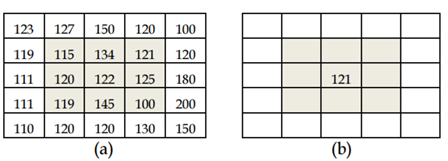
\includegraphics[width=\linewidth]{images/pasted}}
\caption{Averaging of a pixel in median filter}\cite{medianfilterpreprocessing}
\label{fig:Illustration of an OCR system}
\end{figure}

\begin{figure}
\centering
\fbox{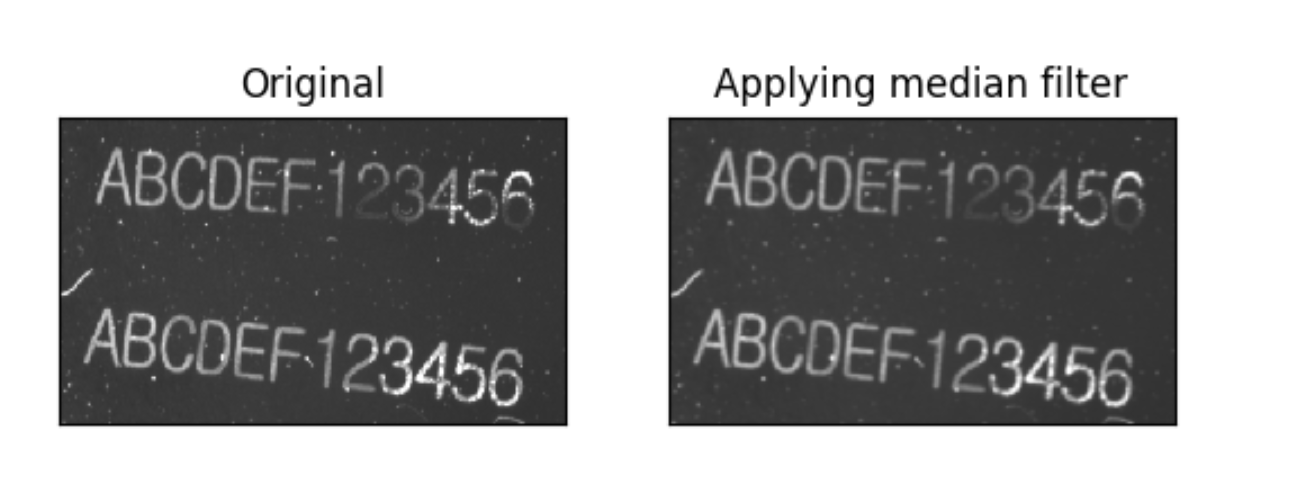
\includegraphics[width=\linewidth]{images/medianfilter}}
\caption{After applying median filter on a scanned image}
\label{fig:Illustration of an OCR system}
\end{figure}

\section{6.Application}

OCR converts images to machine-readable text. That will make it the
initial tool that needs to be used for processing any documents or
simply any written material in a digital image, which has been
captured by a camera\cite{www-ocr-wiki}. It’s output can be stored significantly more
compact than scanned images. But beyond that, it enables us to process
the output information for numerous applications. Examples of these
applications include creating a narrator machine to help the visually
impaired read nondigital documents and signs, or automatic recognition
of automobile number plates.

\section{Acknowledgement}
A very special thanks to Professor Gregor von Laszewski and the
teaching assistants Miao Zhang and Dimitar Nikolov for all the support
and guidance. This project proposal is written during the spring 2017
semester course {I524: Big Data and Open Source Software Projects} at
Indiana University Bloomington.

\bibliography{references}

\end{document}
